\subsubsection{Quản lý tài khoản}
\subsubsubsection{Đăng ký}
\begin{figure}[H]
    \centering
     \includesvg[width=1\textwidth]{Dg_Activity/ManageAccount_Signup.svg}
    \vspace{0.5cm}
    \caption{Biểu đồ activity cho Đăng ký}
    \label{fig:enter-label}
\end{figure}
\subsubsubsection{Đăng nhập}
\begin{figure}[H]
    \centering
     \includesvg[width=1\textwidth]{Dg_Activity/ManageAccount_Login.svg}
    \vspace{0.5cm}
    \caption{Biểu đồ activity cho Đăng nhập}
    \label{fig:enter-label}
\end{figure}
\subsubsubsection{Chỉnh sửa hồ sơ cá nhân}
\begin{figure}[H]
    \centering
     \includesvg[width=1\textwidth]{Dg_Activity/ManageAccount_Profile.svg}
    \vspace{0.5cm}
    \caption{Biểu đồ activity cho Chỉnh sửa hồ sơ cá nhân}
    \label{fig:enter-label}
\end{figure}
\subsubsection{Tích hợp}
\begin{figure}[H]
    \centering
     \includesvg[width=1\textwidth]{Dg_Activity/Activity Diagram-Integration.drawio.svg}
    \vspace{0.5cm}
    \caption{Biểu đồ activity cho Tích hợp}
    \label{fig:enter-label}
\end{figure}

\par Quá trình tạo mã nhúng cho chatbot bắt đầu bằng việc người dùng điều hướng tới trang Tùy chỉnh chatbot. Sau khi truy cập thành công, hệ thống sẽ hiển thị giao diện Tùy chỉnh chatbot và cho phép xem trước giao diện chatbot để đảm bảo rằng thiết kế và các chức năng hoạt động như mong muốn trước khi triển khai. Khi đã hài lòng với bản xem trước, người dùng sẽ nhấn nút Tạo chatbot để hệ thống bắt đầu quá trình tạo mã nhúng. Sau khi hoàn thành, mã nhúng này sau đó sẽ được hiển thị trên giao diện người dùng, cho phép người dùng dễ dàng thao tác. Cuối cùng, người dùng chỉ cần sao chép mã nhúng và dán vào website doanh nghiệp của mình để hoàn tất quá trình tích hợp chatbot.

\subsubsection{Quản lý chatbot}
\subsubsubsection{Báo cáo}
\begin{figure}[H]
    \centering
     \includesvg[width=1\textwidth]{Dg_Activity/Report.svg}
    \vspace{0.5cm}
    \caption{Biểu đồ activity cho Báo cáo}
    \label{fig:enter-label}
\end{figure}
\textbf{Mô tả:}
Ban đầu quản trị viên doanh nghiệp chọn vào nút "Báo cáo" trên thanh điều hướng. Khi đó màn hình sẽ chuyển qua trang Báo cáo và hiển thị các thông số và biểu đồ.
\begin{itemize}
    \item Nếu quản trị viên chọn "Lọc", hệ thống sẽ hiển thị các thông số lọc và quản trị viên chọn một thông số. Khi đó, hệ thống sẽ hiển thị lại các thông số và biểu đồ tương ứng với thông số lọc đó. Rồi sau đó quản trị viên có thể chọn "Lọc" tiếp hoặc chọn "Xuất" hoặc dừng lại.
    \item Nếu quản trị viên chọn "Xuất", hệ thống sẽ hiển thị 2 loại tệp. Sau đó người dùng sẽ phải chọn một và chọn "Xem trước". Hệ thống sẽ hiển thị chế độ xem trước file dưới dạng popup. Nếu người dùng chọn "Tải xuống" thì file sẽ được tải về thiết bị. Còn nếu người dùng chọn "Hủy bỏ" thì hệ thống sẽ đóng popup xem trước.
    \item Nếu quản trị viên không chọn gì thì sẽ kết thúc.
\end{itemize}
\subsubsubsection{Lịch sử hội thoại}
\begin{figure}[H]
    \centering
     \includesvg[width=1\textwidth]{Dg_Activity/Chat.svg}
    \vspace{0.5cm}
    \caption{Biểu đồ activity cho Lịch sử hội thoại}
    \label{fig:enter-label}
\end{figure}
\textbf{Mô tả:}
Ban đầu quản trị viên doanh nghiệp chọn vào nút "Chat" trên thanh điều hướng. Khi đó màn hình sẽ chuyển qua trang Chat và hiển thị danh sách các cuộc hội thoại của khách hàng.
\begin{itemize}
    \item Nếu quản trị viên chọn vào ô tìm kiếm, nhập nội dung tìm kiếm và chọn "Tìm" thì khi đó hệ thống sẽ hiển thị các cuộc hội thoại có tên tương ứng với nội dung tìm kiếm.
    \item Nếu quản trị viên chọn "Lọc", hệ thống sẽ hiển thị các thông số lọc và quản trị viên chọn một thông số. Khi đó, hệ thống sẽ hiển thị lại các cuộc hội thoại tương ứng với thông số lọc đó. 
    \item Nếu quản trị viên chọn "Cần hỗ trợ" thì hệ thống sẽ chỉ hiển thị các cuộc hội thoại mà khách hàng đã gửi yêu cầu hỗ trợ.
\end{itemize}

Sau đó quản trị viên có thể lặp lại các bước trên hoặc chọn xem một cuộc hội thoại. Khi quản trị viên chọn xem một cuộc hội thoại thì hệ thống sẽ hiển thị chi tiết cuộc hội thoại đó.
\subsubsection{Thông báo và cảnh báo}
\begin{figure}[H]
    \centering
     \includesvg[width=1\textwidth]{Dg_Activity/Activity Diagram-Notifications and Alerts.drawio.svg}
    \vspace{0.5cm}
    \caption{Biểu đồ activity cho Thông báo và cảnh báo}
    \label{fig:enter-label}
\end{figure}

\par Quá trình cài đặt thông báo cho người dùng bắt đầu bằng việc người dùng điều hướng tới trang cài đặt thông báo. Khi truy cập thành công, hệ thống sẽ hiển thị trang cài đặt thông báo, cung cấp giao diện để người dùng tùy chỉnh các thiết lập phù hợp với nhu cầu cá nhân.

Tiếp theo, người dùng chọn phương thức nhận thông báo mà họ mong muốn, chẳng hạn như qua email, SMS, hoặc thông báo trực tiếp trên ứng dụng. Sau đó, người dùng thiết lập ngưỡng token LLM hoặc ngưỡng lưu lượng người dùng, nhằm xác định các điều kiện kích hoạt thông báo phù hợp với hoạt động của họ.

Sau khi hoàn tất việc thiết lập các thông số trên, người dùng xác nhận các cài đặt. Hệ thống sẽ áp dụng các cài đặt đã được xác nhận, đảm bảo rằng các thông báo sẽ được gửi đi theo các tùy chọn và ngưỡng đã được thiết lập.

\subsubsection{Quản lý thanh toán}
\begin{figure}[H]
    \centering
     \includesvg[width=1\textwidth]{Dg_Activity/Activity Diagram-Subscription.drawio.svg}
    \vspace{0.5cm}
    \caption{Biểu đồ activity cho Quản lý thanh toán}
    \label{fig:enter-label}
\end{figure}

\par Quá trình đăng ký gói dịch vụ bắt đầu bằng việc người dùng điều hướng tới trang thanh toán. Khi truy cập thành công, hệ thống sẽ hiển thị các gói đăng ký hiện có, cho phép người dùng lựa chọn phù hợp với nhu cầu của mình.

Tiếp theo, người dùng có thể thay đổi hoặc chọn gói đăng ký mới nếu muốn nâng cấp hoặc điều chỉnh dịch vụ. Sau khi lựa chọn gói phù hợp, hệ thống sẽ hiển thị màn hình xác nhận, yêu cầu người dùng xác nhận lựa chọn của mình trước khi tiến hành thanh toán.

Sau khi người dùng xác nhận gói đăng ký, hệ thống sẽ điều hướng tới hệ thống thanh toán để thực hiện giao dịch. Giao diện thanh toán sẽ được hiển thị, nơi người dùng nhập thông tin thanh toán cần thiết như thông tin cá nhân, thông tin thẻ tín dụng hoặc số tài khoản ngân hàng.

Khi người dùng nhập thông tin thanh toán, hệ thống sẽ tiến hành xử lý thanh toán. Nếu thanh toán thành công, hệ thống sẽ kích hoạt gói đăng ký mà người dùng đã chọn, đảm bảo rằng dịch vụ được cung cấp đầy đủ theo gói đã mua. Trong trường hợp thanh toán thất bại, hệ thống sẽ báo lỗi và cho phép người dùng nhập lại thông tin thanh toán hoặc hủy bỏ giao dịch nếu họ quyết định không tiếp tục.


\subsubsection{Tương tác với chatbot}
\subsubsubsection{Phản hồi tin nhắn khách hàng}
\begin{figure}[H]
    \centering
     \includesvg[width=1\textwidth]{Dg_Activity/ReplyCustomerMessage.svg}
    \vspace{0.5cm}
    \caption{Biểu đồ activity cho Phản hồi tin nhắn khách hàng}
    \label{fig:enter-label}
\end{figure}
\textbf{Mô tả:}
Ban đầu quản trị viên doanh nghiệp chọn xem đoạn hội thoại của khách hàng tại trang Chat. Hệ thống sẽ hiển thị màn hình chat với khách hàng đó.
\begin{itemize}
    \item Nếu muốn điền hoặc chỉnh sửa tin nhắn, quản trị viên chọn vào khung điền tin nhắn và nhập nội dung tin nhắn. Khi đó hệ thống sẽ hiển thị đoạn tin nhắn mà quản trị viên đã nhập.
    \item Nếu muốn đính kèm tệp, quản trị viên chọn "Đính kèm tệp đa phương tiện". Khi đó, khung chọn tệp từ thiết bị sẽ được hiển thị. Quản trị viên chọn một tệp và chọn "Tải lên". Hệ thống hiển thị tệp được chọn trên màn hình.
    \item Nếu muốn xóa tệp đã tải lên, quản trị viên chọn "Xóa". Khi đó tệp đó sẽ được xóa khỏi màn hình.
\end{itemize}
Sau đó quản trị viên có thể lặp lại các bước trên. Hoặc nếu đã có tin nhắn và quản trị viên chọn gửi thì hệ thống sẽ hiển thị tin nhắn vừa gửi lên màn hình. Hoặc nếu chưa có tin nhắn thì sẽ dừng lại.
\subsubsubsection{Gửi tin nhắn}
\begin{figure}[H]
    \centering
     \includesvg[width=1\textwidth]{Dg_Activity/SendMessage.svg}
    \vspace{0.5cm}
    \caption{Biểu đồ activity cho Gửi tin nhắn}
    \label{fig:enter-label}
\end{figure}
\textbf{Mô tả:}
Ban đầu khách hàng chọn vào chatbot tại màn hình website của doanh nghiệp. Hệ thống sẽ hiển thị màn hình chatbot.
\begin{itemize}
    \item Nếu muốn điền hoặc chỉnh sửa tin nhắn, khách hàng chọn vào khung điền tin nhắn và nhập nội dung tin nhắn. Khi đó hệ thống sẽ hiển thị đoạn tin nhắn mà khách hàng đã nhập.
    \item Nếu muốn đính kèm tệp, khách hàng chọn "Đính kèm tệp đa phương tiện". Khi đó, khung chọn tệp từ thiết bị sẽ được hiển thị. khách hàng chọn một tệp và chọn "Tải lên". Hệ thống hiển thị tệp được chọn trên màn hình.
    \item Nếu muốn xóa tệp đã tải lên, khách hàng chọn "Xóa". Khi đó tệp đó sẽ được xóa khỏi màn hình.
\end{itemize}
Sau đó khách hàng có thể lặp lại các bước trên. Hoặc nếu đã có tin nhắn và khách hàng chọn gửi thì hệ thống sẽ hiển thị tin nhắn vừa gửi lên màn hình. Đồng thời, hệ thống sẽ tạo và gửi lại tin nhắn phản hồi từ AI Chatbot. Hoặc nếu chưa có tin nhắn thì sẽ dừng lại.
\subsubsubsection{Yêu cầu hỗ trợ}
\begin{figure}[H]
    \centering
    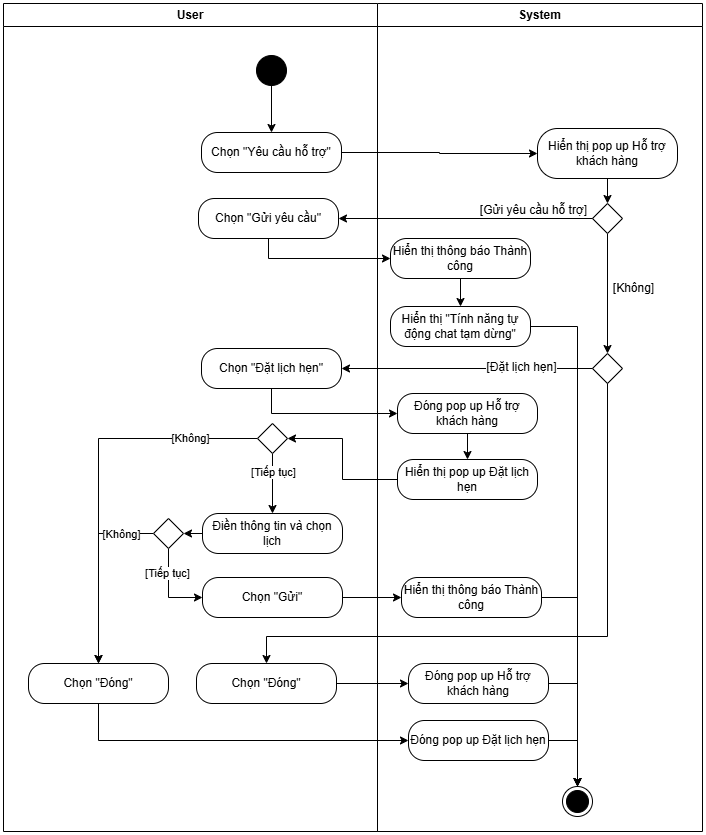
\includegraphics[width=1\textwidth]{Dg_Activity/NeedSupport.png}
    \vspace{0.5cm}
    \caption{Biểu đồ activity cho Yêu cầu hỗ trợ}
    \label{fig:enter-label}
\end{figure}
\textbf{Mô tả:}
Tại màn hình chatbot, khách hàng chọn "Yêu cầu hỗ trợ". Hệ thống sẽ hiển thị popup hỗ trợ khách hàng.
\begin{itemize}
    \item Nếu muốn gửi yêu cầu hỗ trợ, khách hàng chọn "Gửi yêu cầu". Hệ thống sẽ hiển thị thông báo thành công. Khi đó, tính năng tự động chat sẽ tạm dừng.
    \item Nếu muốn đặt lịch hẹn, khách hàng chọn "Đặt lịch hẹn". Hệ thống sẽ đóng popup Hỗ trợ khách hàng và hiển thị popup Đặt lịch hẹn. 
    \begin{itemize}
        \item Nếu muốn tiếp tục, khách hàng điền thông tin và chọn lịch.
        \begin{itemize}
            \item Nếu muốn tiếp tục, khách hàng chọn "Gửi". Hệ thống sẽ hiển thị thông báo thành công.
            \item Nếu không, khách hàng chọn "Đóng".
        \end{itemize}
        \item Nếu không, khách hàng chọn "Đóng".
    \end{itemize}
    Nếu khách hàng chọn "Đóng" thì hệ thống sẽ đóng popup Đặt lịch hẹn.
    \item Nếu khách hàng chọn "Đóng", hệ thống sẽ đóng popup Hỗ trợ khách hàng.
\end{itemize}
\subsubsection{Quản lý lịch hẹn}
\begin{figure}[H]
    \centering
    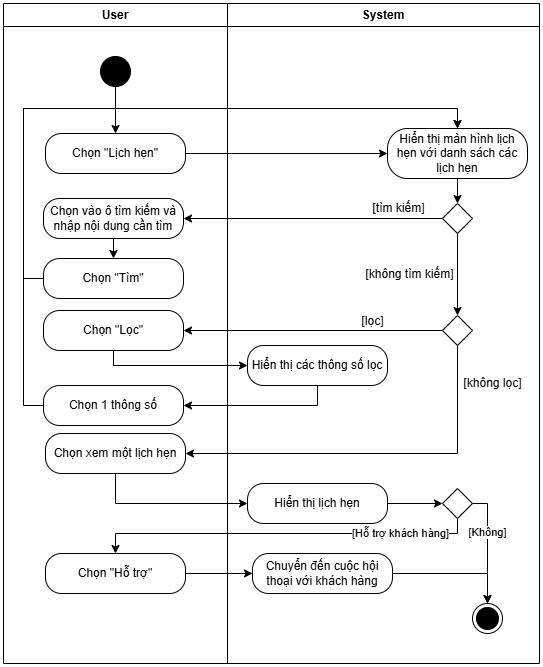
\includegraphics[width=1\textwidth]{Dg_Activity/AppointmentManagement.png}
    \vspace{0.5cm}
    \caption{Biểu đồ activity cho Quản lý lịch hẹn}
    \label{fig:enter-label}
\end{figure}
\textbf{Mô tả:}
Ban đầu quản trị viên doanh nghiệp chọn vào nút "Lịch hẹn" trên thanh điều hướng. Khi đó màn hình sẽ chuyển qua trang Lịch hẹn và hiển thị danh sách các lịch hẹn của khách hàng.
\begin{itemize}
    \item Nếu quản trị viên chọn vào ô tìm kiếm, nhập nội dung tìm kiếm và chọn "Tìm" thì khi đó hệ thống sẽ hiển thị các lịch hẹn có tên tương ứng với nội dung tìm kiếm.
    \item Nếu quản trị viên chọn "Lọc", hệ thống sẽ hiển thị các thông số lọc và quản trị viên chọn một thông số. Khi đó, hệ thống sẽ hiển thị lại các lịch hẹn tương ứng với thông số lọc đó. 
\end{itemize}
Sau đó quản trị viên có thể lặp lại các bước trên hoặc chọn xem một lịch hẹn. Khi quản trị viên chọn xem một lịch hẹn thì hệ thống sẽ hiển thị chi tiết lịch hẹn đó. Ở đó, nếu quản trị viên chọn "Hỗ trợ", hệ thống sẽ chuyển đến cuộc hội thoại với khách hàng. Nếu không thì sẽ dừng lại.


\subsubsection{Đào tạo và tùy chỉnh chatbot}
\subsubsubsection{Tải dữ liệu tri thức}
\begin{figure}[H]
    \centering
     \includesvg[width=1\textwidth]{Dg_Activity/LoadKnowledges.svg}
    \vspace{0.5cm}
    \caption{Biểu đồ activity cho Tải dữ liệu tri thức}
    \label{fig:enter-label}
\end{figure}
\subsubsubsection{Cập nhật dữ liệu tri thức}
\begin{figure}[H]
    \centering
     \includesvg[width=1\textwidth]{Dg_Activity/ModifyKnowledge.svg}
    \vspace{0.5cm}
    \caption{Biểu đồ activity cho Cập nhật dữ liệu tri thức}
    \label{fig:enter-label}
\end{figure}
\subsubsubsection{Gán nhãn dữ liệu tri thức}
\begin{figure}[H]
    \centering
     \includesvg[width=1\textwidth]{Dg_Activity/AssignTopic.svg}
    \vspace{0.5cm}
    \caption{Biểu đồ activity cho Gán nhãn dữ liệu tri thức}
    \label{fig:enter-label}
\end{figure}
\subsubsubsection{Tùy chỉnh chatbot}
\begin{figure}[H]
    \centering
     \includesvg[width=1\textwidth]{Dg_Activity/AdjustBot.svg}
    \vspace{0.5cm}
    \caption{Biểu đồ activity cho Tùy chỉnh chatbot}
    \label{fig:enter-label}
\end{figure}
